Seja $n$ um inteiro positivo. Divide-se um círculo em $n$ setores circulares iguais. Considere o seguinte processo:
\begin{enumerate}[label = (\alph*)]
	\item Inicialmente, coloca-se uma joia em um dos setores e escreve-se o número 0 neste setor.
	\item Na etapa $1$, move-se a joia um setor, no sentido horário, e escreve-se o número $1$ no novo setor onde a joia está.
	\item Na etapa $k$, move-se a joia k setores, no sentido horário, e escreve-se o número $k$ no novo setor onde a joia está.
\end{enumerate}
Terminamos o processo ao fim da etapa $n - 1$. Para quais valores de $n$, ao fim do processo, todos os setores possuem um número escrito?

Abaixo, encontra-se o resultado final do processo para n = 7.

\begin{center}
	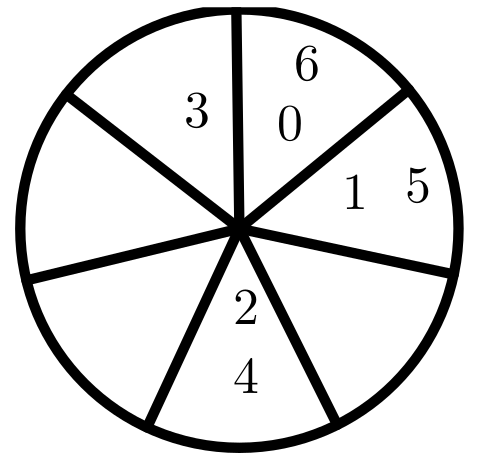
\includegraphics[width = 3cm]{fig1.png}
\end{center}
